\documentclass[10pt,a4paper,twocolumn]{article}
\usepackage[utf8]{inputenc}
\usepackage[english]{babel}
\usepackage{amsmath}
\usepackage{amsfonts}
\usepackage{amssymb}
\usepackage{graphicx}
\usepackage{geometry}
\usepackage{fancyhdr}
\usepackage{listings}
\usepackage{xcolor}
\usepackage{hyperref}
\usepackage[most]{tcolorbox}
\usepackage{enumitem}
\usepackage{booktabs}
\usepackage{caption}
\usepackage{subcaption}
\usepackage{float}
\usepackage{titlesec}
\usepackage{microtype}
\usepackage{parskip}

% Geometry settings
\geometry{
    a4paper,
    top=2cm,
    bottom=2cm,
    left=1.5cm,
    right=1.5cm,
    headsep=0.5cm,
    footskip=1cm
}

\setlength{\headheight}{15pt}
\pagestyle{fancy}
\fancyhf{}
\rhead{Lab 02 - Concurrent Programming}
\lhead{Software Architecture}
\cfoot{\thepage}

\pagenumbering{arabic}

% Code listing settings
\lstset{
    basicstyle=\ttfamily\scriptsize,
    keywordstyle=\color{blue}\bfseries,
    commentstyle=\color{green!60!black}\itshape,
    stringstyle=\color{red},
    showstringspaces=false,
    breaklines=true,
    breakatwhitespace=true,
    frame=leftline,
    framerule=2pt,
    rulecolor=\color{blue!30},
    backgroundcolor=\color{gray!5},
    numbers=left,
    numberstyle=\tiny\color{gray},
    stepnumber=1,
    numbersep=8pt,
    columns=flexible,
    aboveskip=\medskipamount,
    belowskip=\medskipamount,
    xleftmargin=15pt,
    language=Java
}

% Section formatting
\definecolor{darkblue}{RGB}{0,32,96}

\titleformat{\section}
{\color{darkblue}\normalfont\large\bfseries}
{\thesection}{1em}{}

\titleformat{\subsection}
{\color{darkblue}\normalfont\normalsize\bfseries}
{\thesubsection}{1em}{}

\titleformat{\subsubsection}
{\color{darkblue}\normalfont\small\bfseries}
{\thesubsubsection}{1em}{}

% Custom boxes
\newtcolorbox{conceptbox}[1]{
    colback=blue!5!white,
    colframe=blue!75!black,
    colbacktitle=blue!80!black,
    coltitle=white,
    title={\textbf{#1}},
    fonttitle=\bfseries\small,
    boxrule=0.8pt,
    before skip=8pt,
    after skip=8pt,
    left=4pt,
    right=4pt,
    top=6pt,
    bottom=6pt,
    breakable
}

\newtcolorbox{resultbox}[1]{
    colback=green!5!white,
    colframe=green!75!black,
    colbacktitle=green!80!black,
    coltitle=white,
    title={\textbf{#1}},
    fonttitle=\bfseries\small,
    boxrule=0.8pt,
    before skip=8pt,
    after skip=8pt,
    left=4pt,
    right=4pt,
    top=6pt,
    bottom=6pt,
    breakable
}

\newtcolorbox{note}{
    colback=yellow!10!white,
    colframe=orange!75!black,
    colbacktitle=orange!80!black,
    coltitle=white,
    title={\textbf{Important Note}},
    fonttitle=\bfseries\small,
    boxrule=0.8pt,
    before skip=8pt,
    after skip=8pt,
    left=4pt,
    right=4pt,
    top=6pt,
    bottom=6pt,
    breakable
}

\newtcolorbox{warningbox}{
    colback=red!5!white,
    colframe=red!75!black,
    colbacktitle=red!80!black,
    coltitle=white,
    title={\textbf{Race Condition Warning}},
    fonttitle=\bfseries\small,
    boxrule=0.8pt,
    before skip=8pt,
    after skip=8pt,
    left=4pt,
    right=4pt,
    top=6pt,
    bottom=6pt,
    breakable
}

% List formatting
\setlist[itemize]{leftmargin=15pt, itemsep=2pt, parsep=0pt, topsep=5pt}
\setlist[enumerate]{leftmargin=15pt, itemsep=2pt, parsep=0pt, topsep=5pt}

% Caption formatting
\captionsetup{font=small, labelfont=bf, format=hang, indention=0pt, margin=10pt}

% Hyperref setup
\hypersetup{
    colorlinks=true,
    linkcolor=darkblue,
    urlcolor=darkblue,
    citecolor=darkblue,
    pdfborder={0 0 0}
}

% Title page
\title{\vspace{-1cm}
    \begin{center}
        
\includegraphics[width=0.25\textwidth]{media/university_logo.png}
    \end{center}
    \vspace{1.5cm}
    \textbf{\Large Software Architecture Laboratory}\\
    \vspace{1cm}
    \textbf{\huge Laboratory No. 2}\\
    \textbf{\huge Concurrent Programming}\\
    \vspace{1.5cm}
    \large Greyhound Race Simulation with Java 21
}

\author{
    \vspace{2cm}
    \textbf{Students:}\\[0.05cm]
    Andersson David S\'{a}nchez M\'{e}ndez\\[0.3cm]
    Cristian Santiago Pedraza Rodr\'{i}guez\\[0.3cm]
    Elizabeth Correa Su\'{a}rez\\[0.3cm]
    Juan Sebastian Ortega Mu\~{n}oz\\[1.5cm]
    \textbf{Instructor:} Professor Javier Ivan Toquica Barrera\\[0.5cm]
    \textbf{Course:} Software Architecture (ARSW)\\[0.3cm]
    \textbf{Institution:} Escuela Colombiana de Ingenier\'{i}a Julio Garavito\\[2cm]
}

\date{February 6, 2025}

\begin{document}

\onecolumn
\maketitle
\thispagestyle{empty}
\newpage

\tableofcontents
\newpage

\twocolumn

% ============================================
\section{Objective}
% ============================================

This laboratory focuses on implementing thread synchronization mechanisms in a Java Swing application that simulates a greyhound race. The simulation involves multiple concurrent threads representing racing dogs, requiring proper coordination to ensure correct behavior and data consistency.

The specific goals include:

\begin{itemize}
    \item \textbf{Thread Completion}: Ensure the main thread waits for all racing dog threads to finish before displaying final results.
    \item \textbf{Critical Regions}: Protect shared resources (arrival registry) from race conditions using synchronization.
    \item \textbf{Pause/Continue Control}: Implement inter-thread communication for pausing and resuming the race simulation.
\end{itemize}

% ============================================
\section{Problem Description}
% ============================================

The greyhound race simulator presents three main concurrency challenges:

\begin{warningbox}
\begin{enumerate}
    \item \textbf{Premature Results}: The UI displays "final results" before all dogs have finished racing, showing incomplete data.
    \item \textbf{Race Condition}: Multiple dogs finishing simultaneously may corrupt the arrival registry due to unsynchronized access.
    \item \textbf{Control Problem}: No mechanism exists to pause and resume the race in progress.
\end{enumerate}
\end{warningbox}

\subsection{Application Architecture}

The application follows a layered architecture:

\begin{table}[H]
    \centering
    \small
    \begin{tabular}{|l|l|}
        \hline
        \textbf{Package} & \textbf{Responsibility} \\
        \hline
        \texttt{app} & Application entry point \\
        \hline
        \texttt{ui} & Swing GUI components \\
        \hline
        \texttt{threads} & Racing dog threads \\
        \hline
        \texttt{domain} & Arrival registry model \\
        \hline
        \texttt{control} & Race synchronization \\
        \hline
        \texttt{util} & Random number generation \\
        \hline
    \end{tabular}
    \caption{Application package structure}
    \label{tab:packages}
\end{table}

% ============================================
\section{Theoretical Framework}
% ============================================

\subsection{Thread Synchronization with join()}

The \texttt{join()} method blocks the calling thread until the target thread terminates. This provides a barrier synchronization mechanism:

\begin{lstlisting}[caption={Thread Barrier with join()}]
Thread[] workers = new Thread[N];
// Start all threads
for (Thread t : workers) {
    t.start();
}
// Wait for all to complete
for (Thread t : workers) {
    t.join();
}
// All threads have finished
\end{lstlisting}

\begin{note}
The \texttt{join()} method throws \texttt{InterruptedException}, requiring proper exception handling to maintain thread interrupt status.
\end{note}

\subsection{Critical Regions and Synchronized}

A \textbf{critical region} is a code section that accesses shared resources and must be executed atomically. Java's \texttt{synchronized} keyword provides mutual exclusion:

\begin{lstlisting}[caption={Synchronized Method}]
public synchronized void
    registerArrival(String name) {
    // Only one thread can execute
    // this method at a time
    int position = arrivals.size() + 1;
    arrivals.add(name + ": " + position);
}
\end{lstlisting}

The intrinsic lock (monitor) ensures:
\begin{itemize}
    \item \textbf{Mutual Exclusion}: Only one thread holds the lock.
    \item \textbf{Visibility}: Changes are visible to other threads.
    \item \textbf{Atomicity}: The method executes as a single unit.
\end{itemize}

\subsection{Wait/Notify Pattern}

The \texttt{wait()}/\texttt{notifyAll()} mechanism enables inter-thread communication through a shared monitor:

\begin{lstlisting}[caption={Monitor Pattern}]
public class RaceControl {
  private boolean paused = false;
  
  public synchronized void pauseRace() {
    paused = true;
  }
  
  public synchronized void resumeRace() {
    paused = false;
    notifyAll(); // Wake waiting threads
  }
  
  public synchronized void 
      checkPausePoint() throws
        InterruptedException {
    while (paused) {
      wait(); // Release lock and wait
    }
  }
}
\end{lstlisting}

\begin{conceptbox}{Wait/Notify Semantics}
\begin{itemize}
    \item \texttt{wait()}: Releases lock, enters waiting state
    \item \texttt{notify()}: Wakes one waiting thread
    \item \texttt{notifyAll()}: Wakes all waiting threads
    \item Use \texttt{while} loop to guard against spurious wakeups
\end{itemize}
\end{conceptbox}

% ============================================
\section{Implementation}
% ============================================

\subsection{Solution 1: Thread Completion with join()}

The main thread must wait for all dog threads to complete before displaying final results.

\begin{lstlisting}[caption={MainCanodromo.java - join() Implementation}]
// Start all dog threads
carrilSeleccionado.iniciarCarrera();

// Wait for all to finish
for (Galgo galgo : galgos) {
    try {
        galgo.join();
    } catch (InterruptedException e) {
        Thread.currentThread()
            .interrupt();
    }
}

// Now safe to show results
printArrivalOrder();
\end{lstlisting}

\textbf{Why it works:} The \texttt{join()} call blocks the main thread until each individual \texttt{Galgo} thread terminates. Only after all threads have completed does execution continue to display the final results.

\subsection{Solution 2: Critical Region Protection}

The arrival registry is a shared resource accessed by multiple dog threads simultaneously.

\begin{lstlisting}[caption={ArrivalRegistry.java - Synchronized Method}]
public class ArrivalRegistry {
  private List<String> arrivals = 
    new ArrayList<>();
    
  public synchronized void 
      registerArrival(String name) {
    int position = arrivals.size() + 1;
    arrivals.add(
      name + " finished in position " + 
      position);
  }
  
  public synchronized List<String>
      getArrivals() {
    return new ArrayList<>(arrivals);
  }
}
\end{lstlisting}

\textbf{Why it works:} The \texttt{synchronized} keyword ensures that:
\begin{enumerate}
    \item Only one thread can register an arrival at a time.
    \item The position calculation and list addition are atomic.
    \item No two dogs can get the same finishing position.
\end{enumerate}

\subsection{Solution 3: Pause/Continue Synchronization}

The \texttt{RaceControl} class implements the monitor pattern for pausing and resuming the race.

\begin{lstlisting}[caption={RaceControl.java - Full Implementation}]
public class RaceControl {
  private boolean paused = false;
  
  public synchronized void pauseRace() {
    this.paused = true;
  }
  
  public synchronized void resumeRace() {
    this.paused = false;
    notifyAll();
  }
  
  public synchronized void 
      checkPausePoint() 
      throws InterruptedException {
    while (paused) {
      wait();
    }
  }
  
  public synchronized boolean
      isPaused() {
    return paused;
  }
}
\end{lstlisting}

Each dog thread calls \texttt{checkPausePoint()} in its run loop:

\begin{lstlisting}[caption={Galgo.java - Pause Check Integration}]
public void run() {
  while (!finished) {
    try {
      // Check if race is paused
      raceControl.checkPausePoint();
      
      // Continue running
      advance();
      Thread.sleep(randomDelay());
    } catch (InterruptedException e) {
      Thread.currentThread().interrupt();
      break;
    }
  }
}
\end{lstlisting}

% ============================================
\section{Experiments and Results}
% ============================================

\subsection{Race Execution Evidence}

\begin{figure}[H]
    \centering
    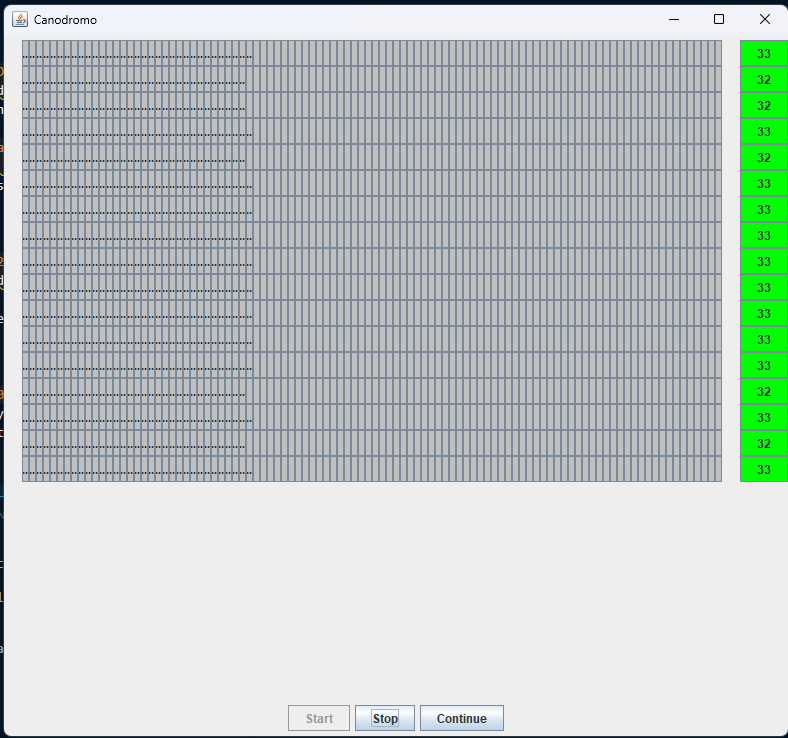
\includegraphics[width=0.45\textwidth]{media/race-running.png}
    \caption{Race in progress: All greyhounds running concurrently in their lanes.}
\end{figure}

\begin{figure}[H]
    \centering
    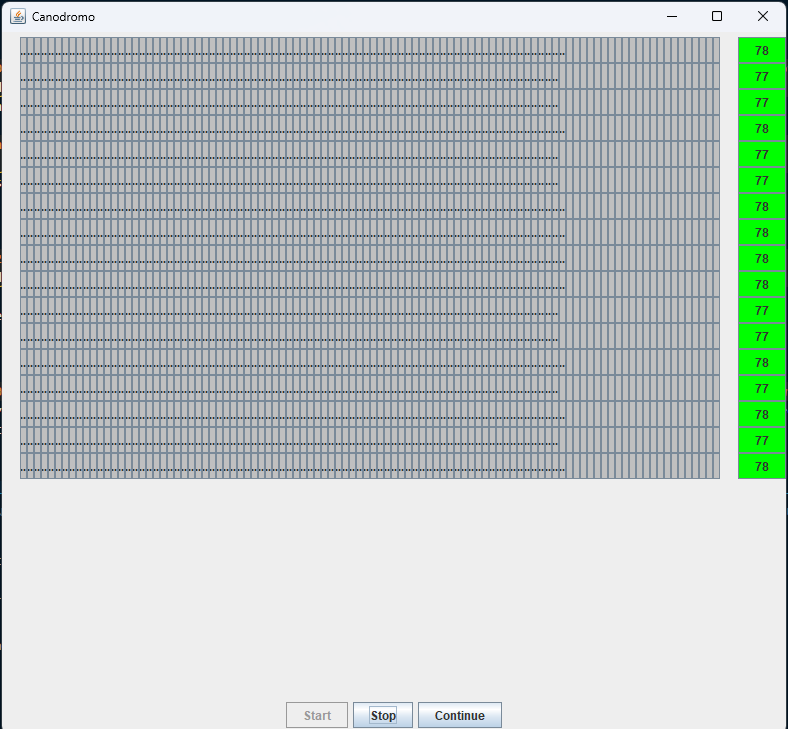
\includegraphics[width=0.45\textwidth]{media/race-paused.png}
    \caption{Race paused: All dogs frozen in place after pressing the Pause button.}
\end{figure}

\begin{figure}[H]
    \centering
    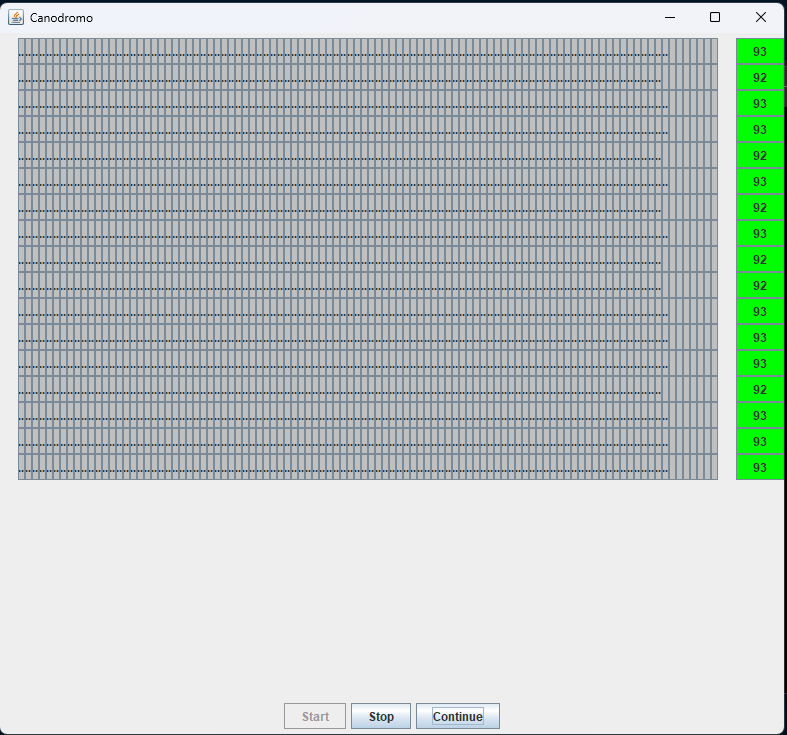
\includegraphics[width=0.45\textwidth]{media/race-resumed.png}
    \caption{Race resumed: Dogs continue from their paused positions after pressing Continue.}
\end{figure}

\subsection{Final Results Display}

\begin{figure}[H]
    \centering
    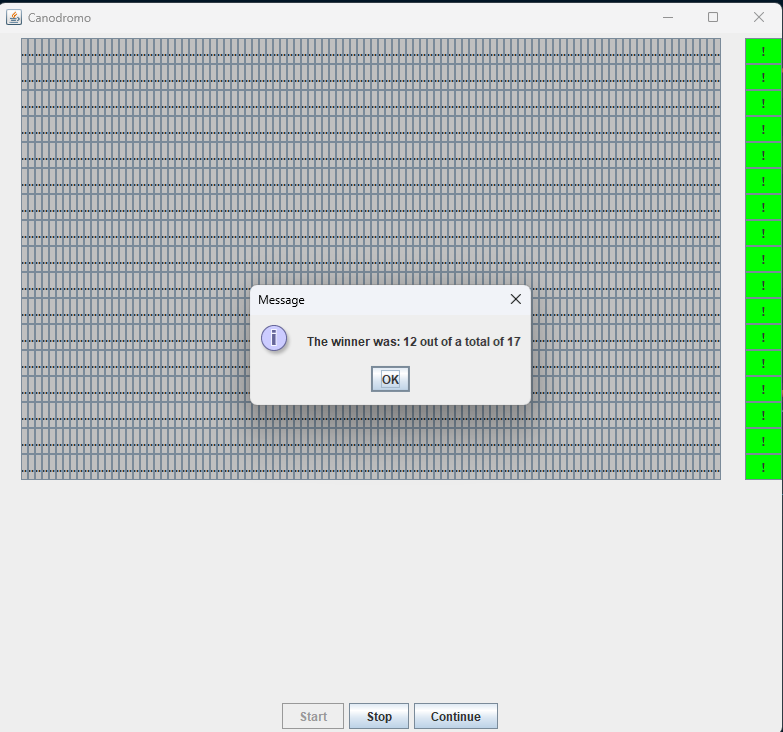
\includegraphics[width=0.45\textwidth]{media/final-results-part1.png}
    \caption{Correct final results: All dogs shown with proper finishing positions (Part 1).}
\end{figure}

\begin{figure}[H]
    \centering
    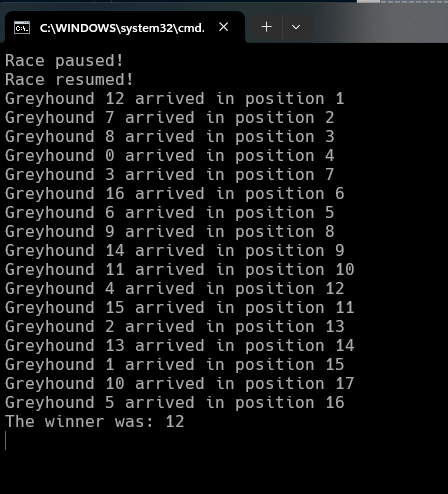
\includegraphics[width=0.45\textwidth]{media/final-results-part2.png}
    \caption{Correct final results: Complete arrival order displayed (Part 2).}
\end{figure}

\subsection{Testing and Coverage}

\begin{figure}[H]
    \centering
    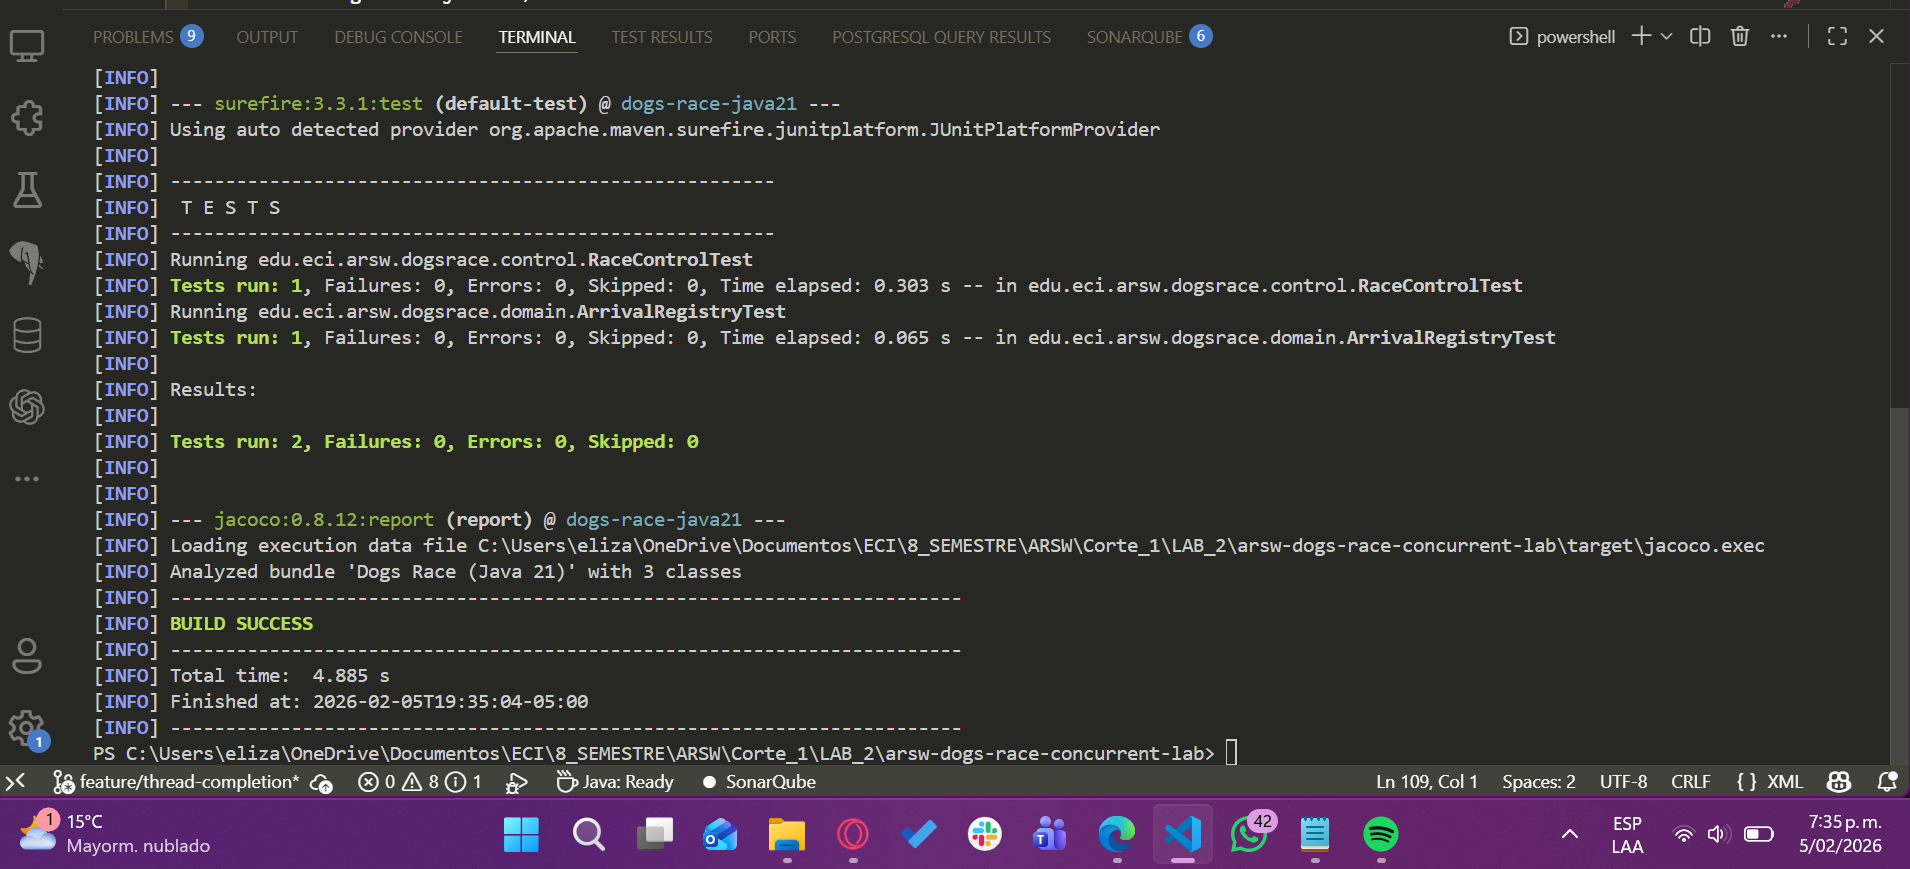
\includegraphics[width=0.45\textwidth]{media/test.png}
    \caption{All unit tests passing: Testing thread-safe arrival registration and race control.}
\end{figure}

\begin{figure}[H]
    \centering
    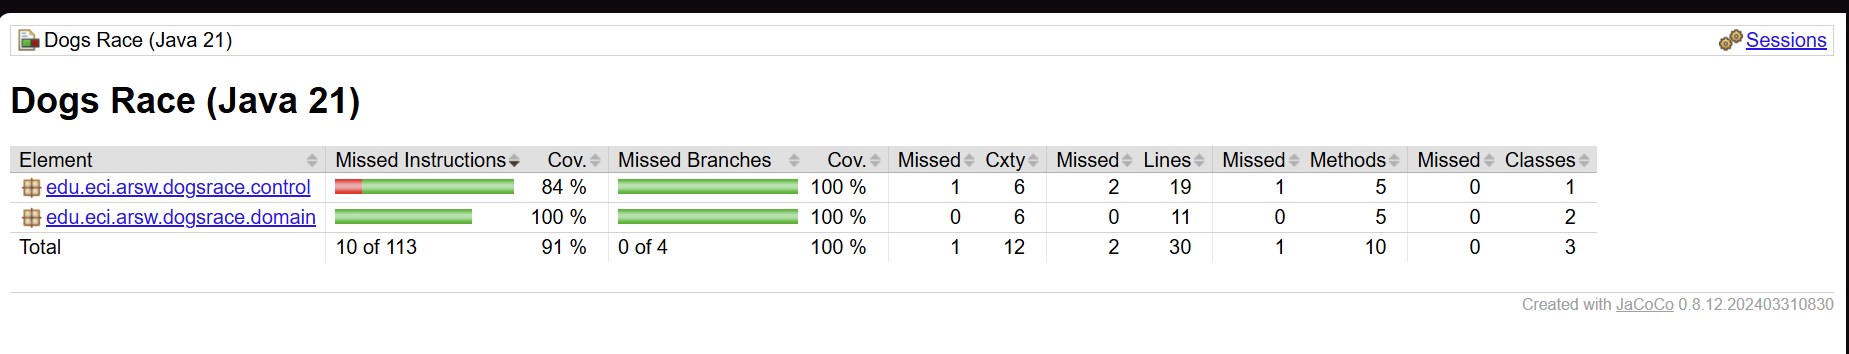
\includegraphics[width=0.45\textwidth]{media/jacoco.png}
    \caption{JaCoCo code coverage report: Coverage targets met for domain and control packages.}
\end{figure}

% ============================================
\section{Synchronization Flow}
% ============================================

The following sequence illustrates the interaction between the UI thread, race control, and dog threads during pause/resume operations:

\begin{enumerate}
    \item \textbf{Normal Operation}: Dog threads run independently, advancing their position.
    \item \textbf{Pause Request}: UI thread calls \texttt{pauseRace()}, setting the flag.
    \item \textbf{Pause Point}: Each dog thread enters \texttt{wait()} at the next \texttt{checkPausePoint()}.
    \item \textbf{Resume Request}: UI thread calls \texttt{resumeRace()}, clearing the flag.
    \item \textbf{Wake Up}: \texttt{notifyAll()} wakes all waiting dog threads.
    \item \textbf{Continue}: Dog threads exit the wait loop and resume racing.
\end{enumerate}

\begin{conceptbox}{Thread States During Synchronization}
\begin{itemize}
    \item \textbf{RUNNABLE}: Dog actively racing
    \item \textbf{WAITING}: Dog paused via \texttt{wait()}
    \item \textbf{BLOCKED}: Dog waiting to acquire monitor lock
    \item \textbf{TERMINATED}: Dog has finished the race
\end{itemize}
\end{conceptbox}

% ============================================
\section{Analysis}
% ============================================

\subsection{Correctness Verification}

The implementation guarantees correctness through:

\begin{itemize}
    \item \textbf{Barrier Synchronization}: \texttt{join()} ensures all threads complete before results display.
    \item \textbf{Mutual Exclusion}: \texttt{synchronized} prevents concurrent registry modifications.
    \item \textbf{Proper Signaling}: \texttt{notifyAll()} ensures all waiting threads are awakened.
    \item \textbf{Spurious Wakeup Protection}: \texttt{while} loop guards the \texttt{wait()} call.
\end{itemize}

\subsection{Thread Safety Analysis}

\begin{table}[H]
    \centering
    \small
    \begin{tabular}{|l|l|l|}
        \hline
        \textbf{Class} & \textbf{Issue} & \textbf{Solution} \\
        \hline
        ArrivalRegistry & Race condition & synchronized \\
        \hline
        RaceControl & Coordination & wait/notify \\
        \hline
        MainCanodromo & Premature output & join() \\
        \hline
    \end{tabular}
    \caption{Thread safety solutions by component}
    \label{tab:safety}
\end{table}

\subsection{Performance Considerations}

\begin{itemize}
    \item \textbf{Lock Contention}: The \texttt{synchronized} method in \texttt{ArrivalRegistry} creates a bottleneck only at race finish, which is acceptable for this use case.
    \item \textbf{Wait Efficiency}: Threads calling \texttt{wait()} release the CPU, avoiding busy-waiting.
    \item \textbf{Scalability}: The solution scales with additional dog threads without modification.
\end{itemize}

% ============================================
\section{Methodology}
% ============================================

\subsection{Test Environment}

Experiments were conducted using the following configuration:

\begin{table}[H]
    \centering
    \begin{tabular}{|l|l|}
        \hline
        \textbf{Component} & \textbf{Specification} \\
        \hline
        Java Version & OpenJDK 21 \\
        \hline
        Build Tool & Maven 3.9+ \\
        \hline
        Test Framework & JUnit 5 \\
        \hline
        Coverage Tool & JaCoCo 0.8.12 \\
        \hline
        Code Analysis & SonarCloud \\
        \hline
        CI/CD & GitHub Actions \\
        \hline
    \end{tabular}
    \caption{Development environment}
    \label{tab:env}
\end{table}

\subsection{Testing Strategy}

Unit tests verify thread-safe behavior:

\begin{lstlisting}[caption={Concurrent Test Example}]
@Test
void testConcurrentArrivals() 
    throws InterruptedException {
  ArrivalRegistry registry = 
    new ArrivalRegistry();
  int numThreads = 100;
  Thread[] threads = new Thread[numThreads];
  
  for (int i = 0; i < numThreads; i++) {
    final String name = "Dog-" + i;
    threads[i] = new Thread(() -> 
      registry.registerArrival(name));
    threads[i].start();
  }
  
  for (Thread t : threads) {
    t.join();
  }
  
  assertEquals(numThreads, 
    registry.getArrivals().size());
}
\end{lstlisting}

% ============================================
\section{Conclusions}
% ============================================

\begin{resultbox}{Key Findings}
\begin{enumerate}
    \item \textbf{join() for Completion}: The \texttt{join()} method provides a simple and effective barrier synchronization for waiting on thread completion.
    
    \item \textbf{synchronized for Safety}: The \texttt{synchronized} keyword protects critical regions, ensuring atomic operations on shared data structures.
    
    \item \textbf{wait/notify for Communication}: The monitor pattern enables efficient inter-thread communication without busy-waiting.
    
    \item \textbf{Design Patterns}: Separating synchronization logic into \texttt{RaceControl} follows the Single Responsibility Principle and improves testability.
    
    \item \textbf{Testing Importance}: Concurrent code requires specific testing strategies to verify thread safety under contention.
\end{enumerate}
\end{resultbox}

\subsection{Lessons Learned}

\begin{itemize}
    \item Always use \texttt{while} loops with \texttt{wait()} to handle spurious wakeups.
    \item Prefer \texttt{notifyAll()} over \texttt{notify()} when multiple threads may be waiting.
    \item Handle \texttt{InterruptedException} properly to preserve interrupt status.
    \item Synchronization should be at the smallest scope necessary to minimize contention.
\end{itemize}

% ============================================
\section{References}
% ============================================

\begin{enumerate}
    \item Goetz, B. et al. (2006). \textit{Java Concurrency in Practice}. Addison-Wesley Professional.
    
    \item Oracle. Java 21 Documentation - Concurrency. \url{https://docs.oracle.com/en/java/javase/21/docs/api/java.base/java/lang/Thread.html}
    
    \item Lea, D. (2000). \textit{Concurrent Programming in Java: Design Principles and Patterns}. Addison-Wesley.
    
    \item Herlihy, M., Shavit, N. (2012). \textit{The Art of Multiprocessor Programming}. Morgan Kaufmann.
\end{enumerate}

\end{document}
